\documentclass[11pt]{article}

% set these commands
\newcommand{\course}{CSCI 534}
\newcommand{\proj}{Homework 01}
\newcommand{\dueDate}{1-28-2021}
\newcommand{\name}{Nathan Stouffer}

\usepackage{../macros}

\newcommand{\pareto}[1]{\rm{Pareto}(#1)}
\newcommand{\conv}[1]{\rm{conv}(#1)}



\begin{document}

\coverpage{02}

\newpage
\section*{Problem 1}

Assume you are given a planar subdivision with $n$ faces in a DCEL. (You may
assume that the planar subdivision does not contain any holes, i.e., there are
no nested faces.) Give pseudo-code for an algorithms that given a vertex $v$ of
the DCEL, outputs all neighbors of $v$. \\\\
\answer
Here is a quick prose description of the algorithm and the pseudo-code is given below in Algorithm \ref{alg:neighbors}.
We are given a vertex $v$ in a DCEL and we want to compute the neighbors of $v$.
We begin by initializing a stack.
Since we have a DCEL, we can get the twin of an incident edge of $v$; label it $e$ ($e$ has $v$ as its destination).
Then push the origin of $e$ to the stack.
Then jump to a new edge $\overline{e}$: the twin of $e$.next.
The edge $\overline{e}$ also has $v$ as its destination so we can push the origin of $\overline{e}$ and repeat this process until we return to the original edge $e$.

\begin{algorithm}
\caption{Computing the neighbors of $v$}
\label{alg:neighbors}
    \begin{algorithmic}[1]
    \Function{Neighbors}{$v$}
        \State nbhd $\gets $ empty stack
        \State $e \gets v$.inc\_edge.twin
        \State nbhd.push($e$.orig)
        \State $\overline{e} \gets$ $e$.next.twin
        \While{$e \neq \overline{e}$}
            \State nbhd.push($\overline{e}$.orig)
            \State $\overline{e} \gets \overline{e}$.next.twin
        \EndWhile
        \State \Return nbhd
    \EndFunction
    \end{algorithmic}
\end{algorithm}

Now we will present a proof of correctness.

\begin{figure}[h]
   \centering
   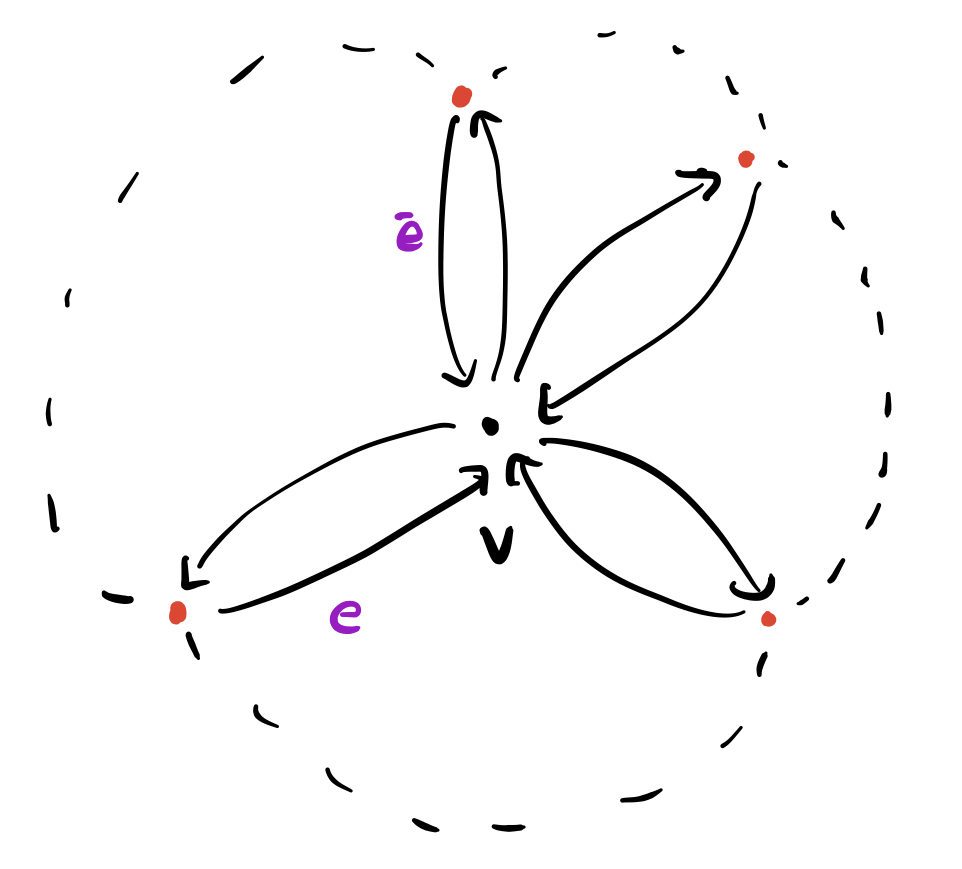
\includegraphics[width=0.3\textwidth]{nbhd}
   \caption{Neighbors of $v$}
\end{figure}

\newpage
\section*{Problem 2}

Assume you are given a planar subdivision of $O(n)$ size in a DCEL. (You may
assume that the planar subdivision does not contain any holes, i.e., there are
no nested faces.) Describe an algorithm that for a given point $p$ in the plane
finds the face in the subdivision that contains it. Your algorithm should run in
$O(n)$ time. You do not have to write pseudo-code, but please make clear what
DCEL operations you are using. Also please make sure the analysis is detailed
enough to justify the $O(n)$ runtime clearly. \\\\
\answer
PROSE DESCRIPTION \\\\
We assume that no vertices in the DCEL share $x$ coordinates and that the point $p$ is entirely inside a face in the DCEL (not a vertex or on an edge).

\begin{algorithm}
\caption{Find the face where $p$ resides}
    \label{alg:findface}
    \begin{algorithmic}[1]
    \Function{FindFace}{DCEL, $p$}
        \For{face in DCEL}
            \State cnt $\gets$ \textsc{CountIntersections}(face, $p$)
            \If{cnt $\equiv 1 \mod 2$}
                \State \Return face
            \EndIf
        \EndFor
    \EndFunction
    \end{algorithmic}

    \begin{algorithmic}[1]
    \Function{CountIntersections}{face, $p$}
        \State cntr $\gets 0$
        \State $h \gets$ horizontal line passing through $p_y$
        \For{each edge $e$ incident to face}
            \State $l \gets$ line passing through the edge $e$
            \State $x \gets$ $x$ coordinate of the intersection between $h$ and $l$
            \If{$x \geq p_x$ and $x$ is between $e$.orig$_x$ and $e$.twin.orig$_x$}
                \State cntr $\gets$ cntr + 1
            \EndIf
        \EndFor
        \State \Return cntr
    \EndFunction
    \end{algorithmic}
\end{algorithm}

We claim the run time of this algorithm is $O(n)$.

PROOF OF CORRECTNESS

\newpage
\section*{Problem 3}

Assume you are given a collection of $n$ circles $\{C_1 , \ldots , C_n \}$ in
$\R^2$, where circle $C_i$ is presented as its center point $q_i = (x_i, y_i)$
and radius $r_i > 0$. Present an $O(n \log n)$ time algorithm that determines
whether any two circles intersect. Note that one circle may be nested within
another without intersecting (see Figure 1). Your algorithm should either output
that there is no intersection, or that there is at least one intersection, and
if so it will output the indices of $i$ and $j$ of two circles $C_i$ and $C_j$
that intersect. Irrespective of the number of intersecting pairs, it need only
output one intersecting pair.

\begin{figure}[h]
    \centering
    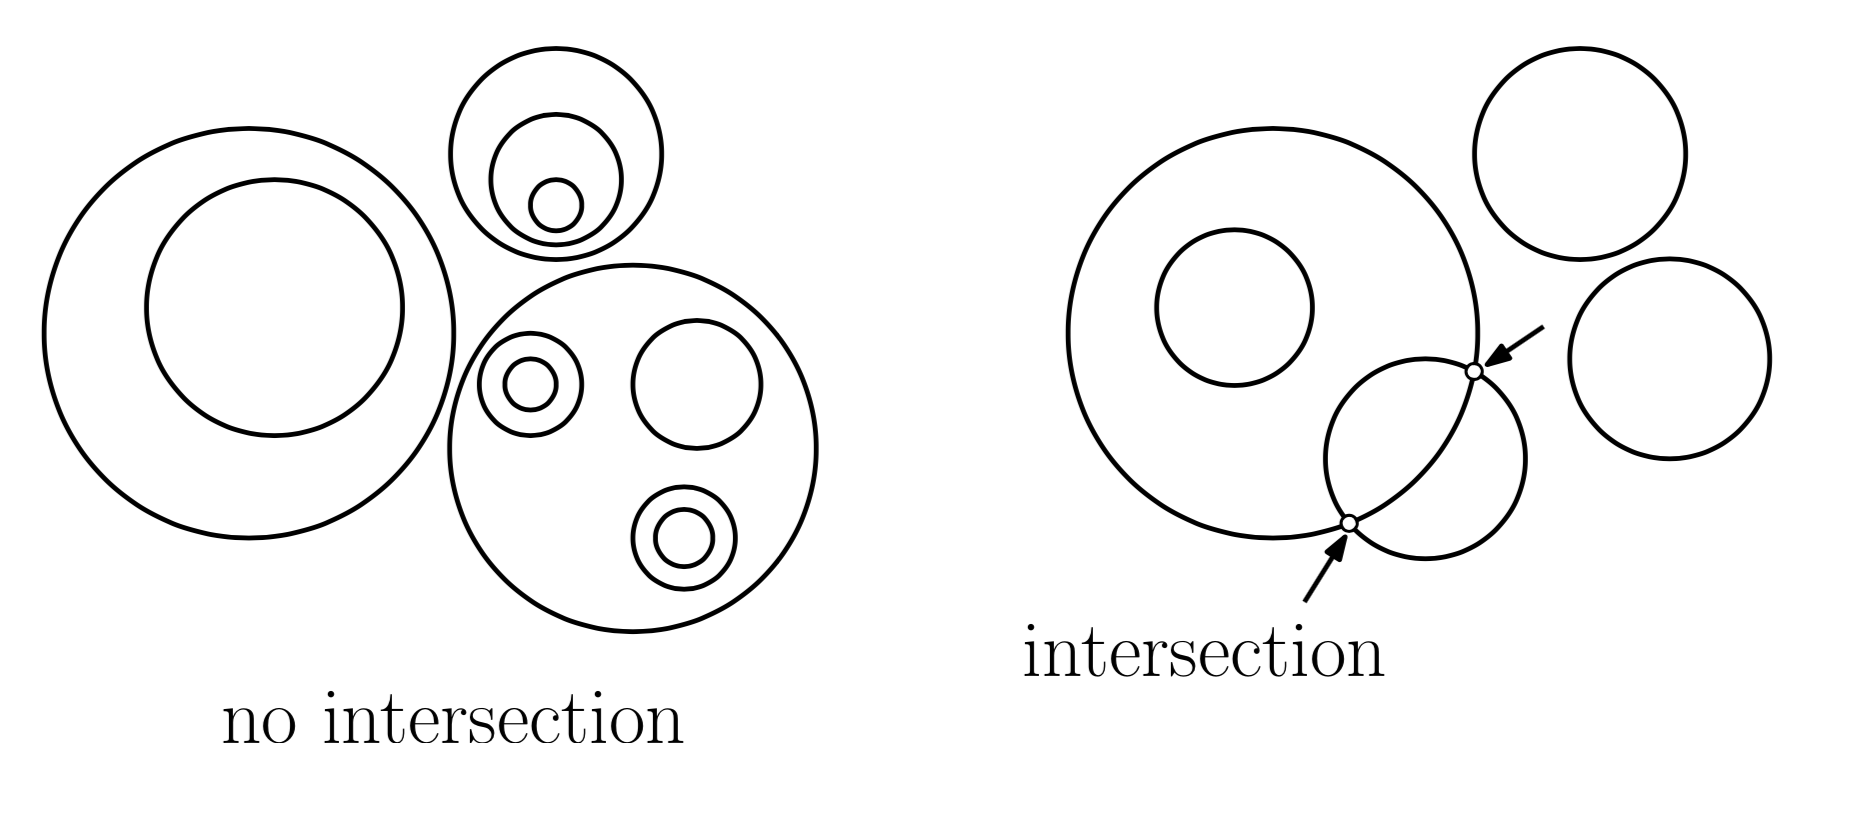
\includegraphics[width=0.75\textwidth]{intersection}
    \caption{Problem 3: Intersection}
\end{figure}

Hint: Use plane-sweep. Explain clearly (1) what the sweep-line status stores and
what data structure is used to store this information and (2) what future events
are stored and what data structure is used. You may assume that you have access
to whatever primitive operations that you need in constant time. For example, if
you want to determine (a) whether two circles intersect, (b) the coordinates of
an intersection, (c) the intersection of a line with a circle, (d) whether a
point is contained within a circle's interior, etc., you may simply assume the
existence of a function that runs in $O(1)$ time. As always, you may make
whatever general-position assumptions you like.

\newpage
\section*{Problem 4}

I have had a few people ask about drawings and making figures.  One tool that I
like to use is Ipe (written by Otfried Cheong).  Ipe allows you to draw content
on layers and show and hide the different layers.  Layers are very helpful if,
for example you want to draw a point set and then show how some data structures
in an algorithm change as you sweep across the point set.
Other vector graphics tools such asIllustrator and Inkscape are also quite good.

Setup Ipe \url{http://ipe.otfried.org/}, Illustrator, or Inkscape
(or another vector graphics tool)
to create 3 images of the state of the sweep line algorithm
described in problem 3.

% \section*{Tips and Acknowledgements}
%
% For drawing pictures with Ipe, check out the layer pallet (in the bottom
% left hand corner).  It is very helpful for creating algorithm animations.
%
% {\bf Acknowledgements:} Homework problems adapted from assignments of David
% Mount and Carola Wenk.

\end{document}
